
\documentclass[12pt,a4paper, oneside]{book}
\usepackage[utf8]{inputenc}
\usepackage{amsmath}
\usepackage{amsfonts}
\usepackage{amssymb}
\usepackage{graphicx}

%allows tables to span across pages
\usepackage{longtable}

\usepackage{mathpazo} % Palatino font

%This is the linux path
%\graphicspath{{/home/wasabi/Documents/LaTex-Documents/ba-latex-code/images/}} % sets image folder
%This is the mac path
%
\graphicspath{{/Users/drexl/Documents/ba-latex-code/images/}} % sets image folder
%windows path
\graphicspath{{C:\\Users\\drexl\\Projects\\ba-latex-code\\images\\}}

%added this package to frame (add boxes) around my equations. Just a personal favorite of mine.
\usepackage{framed}
%to use?

%This prevents placing floats before a section.
\usepackage[section]{placeins}

%added this package, so i could float non-traditional objects
%like lists. By default, only tables and images can be floating objects.
%needed to do this, so that I could use captions on my equations.
\usepackage{float}

%used for creating nice looking definition section of our SRS
\usepackage{enumitem}% http://ctan.org/pkg/enumitem

%used to add captions
%to float text around an image
\usepackage{wrapfig}
\usepackage[section]{placeins}
\usepackage{caption}

% Used for displaying code blocks
\usepackage{minted}
% surround code with box
\usepackage{tcolorbox}
\usepackage{etoolbox}

\BeforeBeginEnvironment{minted}{\begin{tcolorbox}}%
\AfterEndEnvironment{minted}{\end{tcolorbox}}%

%new command added to change Bibliography title to References
\renewcommand{\bibname}{References}

\usepackage[left=2cm,right=2cm,top=3cm,bottom=3cm]{geometry}

\begin{document}

%----------------------------------------------------------------------------------------
%	TITLE PAGE
%----------------------------------------------------------------------------------------

\begin{titlepage} % Suppresses displaying the page number on the title page and the subsequent page counts as page 1
	\newcommand{\HRule}{\rule{\linewidth}{0.5mm}} % Defines a new command for horizontal lines, change thickness here
	
	\center % Centre everything on the page
	
	%------------------------------------------------
	%	Headings
	%------------------------------------------------
	
	%\textsc{\LARGE Hochschule für Technik \& Wirtschaft Berlin}\\[1.5cm] % Main heading such as the name of your university/college
		
\includegraphics[width=0.9\textwidth]{/Users/esteban/Projects/ba-latex-code/images/logo.png}\\[1cm] % Include a department/university logo - this will require the graphicx package
	
	\textsc{\Large Bachelorarbeit}\\[0.5cm] % Major heading such as course name
	
	\textsc{\large Fachbereich 4: Internationale Medieninformatik}\\[0.5cm] % Minor heading such as course title
	
	%------------------------------------------------
	%	Title
	%------------------------------------------------
	
	\HRule\\[0.4cm]
	
	{\huge\bfseries Thunderbird Add-on: 'One Time Password/Pad' Encryption}\\[0.4cm] % Title of your document
	
	\HRule\\[1.5cm]
	
	%------------------------------------------------
	%	Author(s)
	%------------------------------------------------
	
	\begin{minipage}{0.4\textwidth}
		\begin{flushleft}
			\large
			\textit{Student}\\
			Esteban \textsc{Licea} % Your name
		\end{flushleft}
	\end{minipage}
	~
	\begin{minipage}{0.4\textwidth}
		\begin{flushright}
			\large
			\textit{Mentor/Supervisor}\\
			Prof. Dr. Debora \textsc{Weber-Wulff} % Supervisor's name
		\end{flushright}
	\end{minipage}
	
	% If you don't want a supervisor, uncomment the two lines below and comment the code above
	%{\large\textit{Author}}\\
	%John \textsc{Smith} % Your name
	
	%------------------------------------------------
	%	Date
	%------------------------------------------------
	
	\vfill\vfill\vfill % Position the date 3/4 down the remaining page
	
	{\large\today} % Date, change the \today to a set date if you want to be precise
	
	%------------------------------------------------
	%	Logo
	%------------------------------------------------
	
	%\vfill\vfill

	 
	%----------------------------------------------------------------------------------------
	
	\vfill % Push the date up 1/4 of the remaining page
	
\end{titlepage}

\newpage
\section{Abstract}
%\paragraph{TBD. Fill this out in 3-4 sentences what the report describes}

\paragraph{The developer describes the steps in researching and developing a Thunderbird Add-on that offers E2EE, without the need for key changes, i.e. without PGP. The developed software will allow one user to exchange a keyword/password with another user, encipher a message with that keyword/password, and the other user will be able to decipher to message with that password.}

\newpage

\section{Acknowledgements}

\paragraph{First off, I need to give credit to my partner and child, who did their best to limit distractions and allow me to complete this project. Without their continued support and love, this project would have been a great deal more complicated.}

\paragraph{Secondly, I need to give special mention to John Bieling, an adminitrative Thunderbird Developer, who gave invaluable guidance to many roadblocks and issues I had along the way. He was always able to point me in the right direction, and without his help this project would have not been completed.}

\tableofcontents

% This if from notes in talking with Dr. Weber-Wulff on May 9th.
% Audience is someone holding a bachelor's in Computer Science
% I don't need to tell them what HTML is, or a programming language
% I do however need to give a quick view of various other aspect of
% the report that may be more specific, in my case the Thunderbird Webextensions API
% encryption, etc..

% Do I need to mention motivation? Email and Email client can go under that.
% what is another word for motivation

% Also, according to Dr. Weber-Wulff, the rule of them for quoting works is thus
% if it's something EVERYONE knows, then I don't need to note it.

% On the other hand, if I do need to quote it think of this:

% { a Beginning
% } an End
% => and a Source

\chapter{Introduction}

\paragraph{The digital age has fully absorbed our societies. We do everything in some form or another of digital media: create art, science, communicate, create and share memories, play games, and write thesis reports with our computers. There is basically no limit to what people do with their computers.}

\paragraph{Proportional to this growth, the internet's influence on our lives has also ballooned. Our activities have been pushed more and more online, onto the cloud. Originally, few bothered to think about privacy. Most damaging, perhaps, was the erroneous expectation of private communication. Edward Snowden's revelations about the "Five Eyes" intelligence alliance, and cooperation in the collection of all online communication, social media, and phone data. No online communication has been considered safe ever since.}


\section{Problem}

\paragraph{Mozilla has tried to support end-to-end encryption (E2EE? for a long time, it has been faced with a major obstacles:}

\begin{itemize}
\item Setting the PGP add-on Enigmail was too technical
\item Generating keys was too technical
\item Even if conditions 1. \& 2. were fulfilled, it was especially uncommon that anyone else you would want to converse with would have gone through the trouble to setup a client or keys for themselves
\item Mozilla is in the process of using OpenPGP build-in to the client, but that also has problems, most obviously, you again need new keys (granted easier to setup this time)
\item and, again, both people must have generated keys (again
\end{itemize}

\paragraph{Thus, the problem: How can Alice send an encrypted email to someone that does not have any type of public key available?}


\section{Context}
\paragraph{While PGP has existed for years, it is predicated on the exchange of public keys. In clear text, there is a technical requirement to create and exchange keys, and installation of any additional required client software that most average users do not have the patience to complete. Originally, Thunderbird relied on an add-on, Enigmail, to create, manage, and exchange keys.}

\paragraph{Starting with Thunderbird 78, Mozilla implemented OpenPGP as part of it's core client software, and dropped support for all add-ons not using MailExtensions (which includes Enigmail). However, the feature is disabled by default, and is still considered a work in progress. All other add-ons found on Thunderbird's extensions page or searching through Github were considered to be in a testing or experimental phase.}

\section{My solution to the problem}
%3. Introduce my current research
\paragraph{This project will implement of an Email Add-on that will allow end-to-end encrypted (E2EE) communication. More specifically, it will focus on the Mozilla Thunderbird client, for the simple fact that I have personally used it for over ten years, it's free, open-source, and cross platform. While I grant that not everyone uses Thunderbird, at least there should be no shortage of users, and theoretically anyone can get it easily, for free.}

\paragraph{Ultimately, this project aims to offer a simple, albeit \emph{not} perfect solution for those interested in privacy, that don't have the technical expertise to engage in key creation, exchanges or have zero knowledge about encryption. The \author{Esteban Licea} will demonstrate the advantages and disadvantages of various implementations strategies, and implement a solution that offers, hopefully, a viable encryption option that will fulfill some use cases.}

\section{Methods applied}
%1. Establish your territory - begin to elaborate what your topic is about

%2. Establish a niche - why did i pick my topic in the first place



\paragraph{The methods and tools used to solve this research inquiry will include:}

\begin{enumerate}
\item Literature either in the form of online or paper publications, i.e. books
\item Online learning resources
\item Thunderbird and JS Encryption APIs
\item Guidance from Mentors
\item Visual Studio Code for code production
\item Github for Source Code and Thesis code management
\item Latex for writing the Thesis
\item Jira for project management, i.e. Kanban board, sprints, and road maps
\end{enumerate}

\paragraph{After the research has been completed, all coding will proceed using a test driven development approach. Thunderbird Add-ons are based on MailExtension technology, which are created using the follow standard languages:}

\begin{enumerate}
\item HTML
\item CSS
\item Javascript
\end{enumerate}











\chapter{Cryptography}
%Quick overview of cryptography

\section{Algorithm selection overview}
%Which encrypting plan will I use?

\subsection{Symmetric key encryption}
\paragraph{Selecting an algorithm, among so many, was pretty straightforward given my use case, but I wanted to show my thought processes. Firstly, there are two fundamental paths for selecting an encryption algorithm. The selection between \emph{asymmetric} and \emph{symmetric} key encryption is the initial decision.}

\begin{enumerate}
\item Asymmetric-key cryptography: A public and private key are created by both people wanting to exchange encrypted emails. This is the most secure and most commonly implementated encryption available, popularly known as "public-key encryption." Examples encryption key algorithms used include RSA and Diffe-Hellman-Merkle.
There are challenges though:\cite{book0}
\begin{enumerate}
\item Both parties need to create their own keys
\item Keys need to be exchanged, i.e. a person has to be acute enough to search for the other person's public key -- assuming one even exists
\item Additional client software is also often required
\end{enumerate}
\item Symmetric-key Encryption: use the same key for both encryption and decryption\cite[p. 155]{book1}
\begin{enumerate}
\item The primary drawback is that both parties will need to exchange that key, often times in the form of a password.
\end{enumerate}
\end{enumerate}

\paragraph{The goal of this project is \emph{ease of use} (at the cost of security), so our choice is clear: symmetric-key encryption.}

\subsection{Block vs. Stream cipher encryption}
\paragraph{Next, we need to decide between a block cipher or a stream cipher. As Bruce Schneier defines the two in his book "Applied Cryptography: Protocols, Algorithms in C" as:}

\begin{quote}
There are two basic types of symmetric algorithms: block ciphers and stream ciphers. Block ciphers
operate on blocks of plaintext and ciphertext—usually of 64 bits but sometimes longer. Stream
ciphers operate on streams of plaintext and ciphertext one bit or byte (sometimes even one 32-bit
word) at a time. With a block cipher, the same plaintext block will always encrypt to the same
ciphertext block, using the same key. With a stream cipher, the same plaintext bit or byte will
encrypt to a different bit or byte every time it is encrypted.\cite[p. 12]{book2}
\end{quote}
\paragraph{The advantages of a stream ciphers:}\footnote{https://crashtest-security.com/block-cipher-vs-stream-cipher/}

%TODO resume here, giving highlight to stream without reason. Instead, mention that by now, mixed algorithms are also possible -if not, prevalent.

\begin{itemize}
\item bit or byte at a time encryption
\item speed of encryption/decryption
\end{itemize}

\paragraph{are more appropriate for hardware implementations.}

\paragraph{According to Bruce Schneier, block ciphers are more suitable for software implementation as they are easier to implement, avoid time-consuming bit manipulations, and operate on computer sized blocks.}\cite[p. 172]{book2}

\subsection{Block cipher selection}
\paragraph{There are many block ciphers to choose from, these are just some of the most popular:}\cite{book3}
\begin{enumerate}
\item Digital Encryption Standard(DES): DES is a symmetric key block cipher that uses 64-bit blocks, but it has been found vulnerable to powerful attacks. This is the reason the use of DES is on a decline. 
\item Triple DES:This symmetric key cipher uses three keys to perform encryption-decryption-encryption. It is more secure than the original DES cipher but as compared to other modern algorithms, triple DES is quite slow and inefficient. 
\item Advanced Encryption Standard(AES): AES has superseded the DES algorithm and has been adopted by the U.S. government. It is a symmetric key cipher and uses blocks in multiple 32 bits with minimum length fixed at 128 bits and maximum at 256 bits. The algorithm used for AES, was originally named Rijndael.\footnote{The winners of the AES competition were two Belgians: Vincent Rijmen, Joan Daemen, thus the algorithm's name: "\textbf{Ri}n\textbf{jdae}l"}
\item Blowfish: Blowfish is a symmetric key block cipher with a block size of 64 and a key length varying from 32 bits to 448 bits. It is unpatented, and the algorithm is available in the public domain. 
\item Twofish: Twofish is also a symmetric key block cipher with a block size of 128 bits and key sizes up to 256 bits. It is slower than AES for 128 bits but faster for 256 bits. It is also unpatented and the algorithm is freely available in the public domain.
\end{enumerate}

\paragraph{But, after an overall account of the block enciphers available, the author decided there is really only one reasonable choice: the Advanced Encryption Standard (AES). This decision is based }

\section{Advanced Encryption Standard (AES)}

\paragraph{AES is basically the only choice for a block cipher scheme. It has been the industry standard for the past 20 years, even used by the U.S. government.}\cite{book4}

%TODO what is my reasoning for selecting AES?
%AES is derived from a competition from 1997, spanning world wide competitors. A belgian team won, an
% Which mode of choose, why??

%Describe the mathematics involved in the Algorithm.

%Start with Field Theory - Galois 
\paragraph{The foundation upon which the AES standard is built is based on Field Theory. More precisely, the theory of \emph{Galois Fields}. Explain basically what a Galois field is here.}
%TODO What is a Galois field, what makes it special? Do irreducible polynomials go here?

%Modulo of a irreducible polynomial
\paragraph{Modulo arithmetic is commonly used in Computer science, and needs little explanation. It is the amount left over by the division of two integers, commonly known as the \emph{remainder}. It is written as: $11 MOD 4 = 3$.}

\paragraph{We'll also need to remember polynomials from basic algebra. More precisely, the mathematics upon them, with special interest on the coefficients. Next, we will recall the division of polynomials, and the special set of polynomial divisors name \emph{irreducible polynomials.} These are polynomials that ???}
%TODO Explain in more detail what irreducible polynimals are, and the important ones for this algorithm.

\paragraph{Now, that we have an reviewed all the required mathematics,}

\begin{enumerate}
\item Galois Fields
\item Polynomials, and their division
\item Irreducible polynomials
\item Modulo arithmetic
\end{enumerate}

\paragraph{we can begin with the genius of the algorithm.}

%TODO what is or how is key expansion done??

%XOR with key??
\subsection{Step One:}
\paragraph{Adding the key to the mix, the longer the key the better!}


%Byte substitution - bit shifting?
\subsection{"SubBytes" or byte substitution}
\paragraph{What happens here is the that bytes get shifted?}



%Row Shifting
\subsection{ShiftRows or the rows are shifted}
\paragraph{The rows are shifted..}


%Column mixing??
\subsection{MixColums or the columns are mixed}
\paragraph{Here, the columns are mixed in "this" manner.}

%Add round key??
\subsection{AddRoundKey or the key (which key, partial) is re-added}
\paragraph{"This" key is re-added, xor'd? Which key, back to the field.}


%Algorithm (all the above) is repeated 9-13 times, depending on bit level of encryption.
\subsection{The process is repeated x number of times.}


% Goal to achieve Diffusion and Confusion.
\subsection{AES algorithm summary}
\paragraph{The goal of the algorithm is to insert confusion and diffusion into the field, over and over. And, the algorithm is just reversed to retrieve the plain text. The algorithm was fast in 2001, when it was introduced, but now, 20 years later, it is built into all modern desktop CPUs (at least Intel and AMD), so it's blazingly fast.}

%TODO fix the spacing of this image!
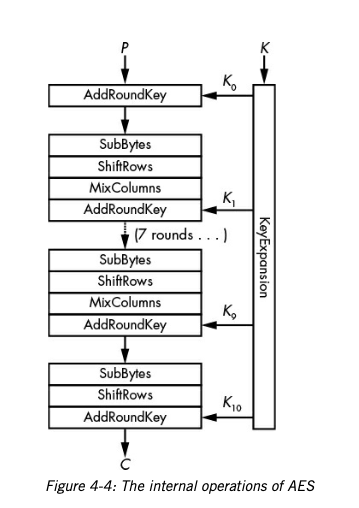
\includegraphics[width=0.9\textwidth]{AES-image.png}

\chapter{Implementation}



\section{Javascript Cryptography}

\paragraph{The developer decided that the best solution for the cryptography implementation was the utilization of a pre-existing cryptography library.}

\paragraph{For this task, there were three necessary conditions that had to be met:}

\begin{itemize}
\item A clear, easily identifiable, and reputable source/owners
\item Existing, easily obtainable, and comprehensive documentation
\item Open source, easily available code
\end{itemize}

\paragraph{and, slightly less important, actively maintained.}

\paragraph{Meeting the above criteria was not as simple as it would seem. There were many options that met some of the conditions, but meeting them all was more challenging. Ultimately, however, the researcher was satisfied with the Stanford Javascript Crypto Library (SJCL), as it met all the above conditions. Additionally, it appeared to be well developed, and maintained.}\cite[Website]{SJCL}

\paragraph{The usage is pretty straight forward, and will work for this implementation. Simply linking the javascript source in the html file (See reference figure: \ref{fig: exampleSJCL_html}).:}

\begin{figure}[H]
\begin{minted}[breaklines]{html}
<!DOCTYPE html>
<html>
<head>
    <meta charset="utf-8"/>
    <script src="http://bitwiseshiftleft.github.io/sjcl/sjcl.js"></script>
</head>
</html>
\end{minted}
\caption{\label{fig: exampleSJCL_html} Example of linking SJCL in HTML}
\end{figure}

\paragraph{and, the javascript can simply be used as follows (See reference figure: \ref{fig: exampleSJCL_js}):}

\begin{figure}[H]
\centering
\begin{minted}[breaklines]{javascript}
var ciphertext = sjcl.encrypt("reallyHardPasswordNoOneCouldEveryGuess", "Hello World!");
var plaintext = sjcl.decrypt("reallyHardPasswordNoOneCouldEveryGuess", ciphertext);
console.log("plain text: " + plaintext);
console.log("cipher text: " + ciphertext);
console.log("plain text - again!: " + plaintext);
\end{minted}
\caption{\label{fig: exampleSJCL_js} Example of javascript SJCL}
\end{figure}

\paragraph{giving the following result (See reference figure: \ref{fig: exampleSJCL}):}

\begin{figure}[H]
\centering
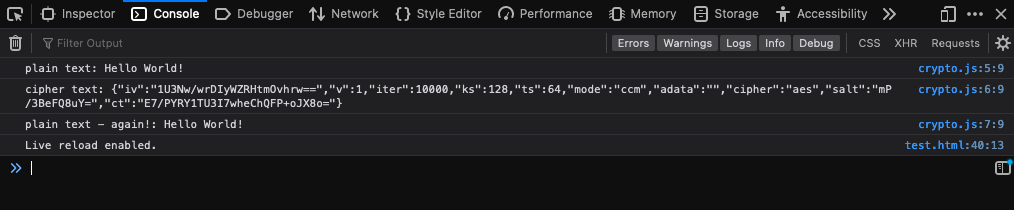
\includegraphics[width=0.9\textwidth]{exampleSJCL.png}
\caption{\label{fig: exampleSJCL} Example output to Firefox console}
\end{figure}

\paragraph{The usage is pretty straight forward, and will meet our needs.}

\section{WebExtensions}

\paragraph{WebExtensions are web technology built with the tools that are natural to any web developer: HTML, CSS, and Javascript. Each extension must have a \emph{manifest.json} file, which essentially hold all the vital information as to the author of the software, permissions required to use the add-on, the software version, and so on.} \cite[Webpage]{WebEx}

\paragraph{Starting with the release of Thunderbird version 68 (August 2019), Thunderbird moved to only support WebExtensions for add-ons and themes development, with all previous versions no longer working. Even the long standing Enigmail cryptography add-on that the author used for years, no longer functioned.}

\paragraph{Here is an image from Mozilla's Thunderbird Add-on Webpage that gives a quick glance of how the extensions might look like.}\footnote{Source: same webpage as noted above.}


\begin{figure}[H]
\centering
\includegraphics[width=0.9\textwidth]{webEx.png}
\caption{\label{fig: webEx} WebExtension overview}
\end{figure}


\section{Implementation Details}
\paragraph{But, lets dive right in and get started. As we step through the development, it will become more clear.}

\subsection{Creating a button}

\paragraph{First, we'll create a button that will appear in the "Compose Window," the window that appears when you start to write an email.}

\paragraph{Before add-on implementation:}

%add image here
%add Image
\begin{figure}[H]
    \centering
    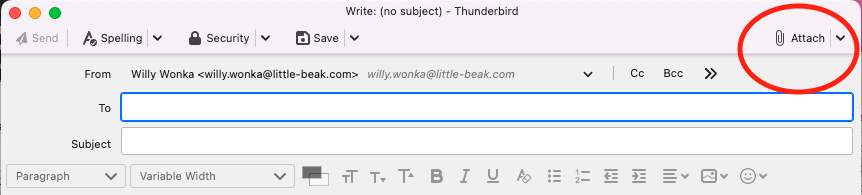
\includegraphics[width=0.9\textwidth]{ComposeWindow_No_Button.png}
    \caption{\label{fig: noButton} Normal compose window}
\end{figure}

\paragraph{with add-on button implemented.}

%add image
%add Image
\begin{figure}[H]
    \centering
    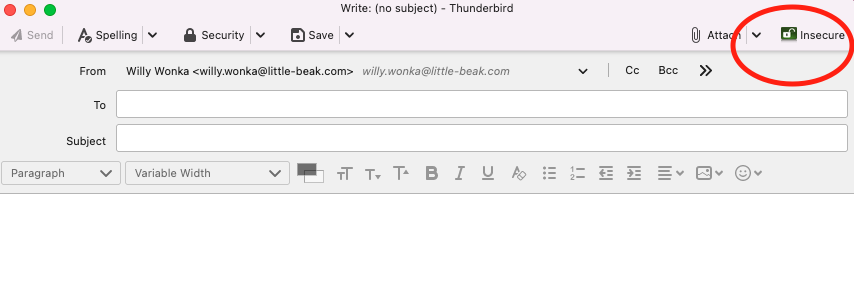
\includegraphics[width=0.9\textwidth]{ComposeWindowButtonInsecure.png}
    \caption{\label{fig: withButton} Button added to the compose window.}
\end{figure}

\paragraph{And, here is the manifest.json file that was created for this button. Most of the references in the manifest.json file, are, well manifest. The only thing of interest is the manifest version of 2. Apparently, it has to be 2, and it always is 2. The rest provide information about the add-on, location of images used, and the permissions required for the add-on to function. (See reference figure: \ref{fig: basic_manifest.json}).:}

%add code here
\begin{figure}[H]
\centering
\begin{minted}[breaklines]{javascript}
{
    "manifest_version": 2,
    "name": "Crypto add-on",
    "description": "A password AES cryptographic addon",
    "version": "1.0",
    "author": "Esteban Licea",
    "applications": {
        "gecko": {
            "id": "esteban@little-beak.com",
            "strict_min_version": "78.0"
        }
    },
    "compose_action": {
        "default_title": "Insecure",
        "default_icon": "images/unlocked_64px.png"
    },
    "permissions": [
        "menus"
    ],
    "icons": {
        "64": "images/unlocked_64px.png",
        "32": "images/unlocked_32px.png",
        "16": "images/unlocked_16px.png"
    }
}
\end{minted}
\caption{\label{fig: basic_manifest.json} Basic manifest.json file}
\end{figure}

%% I was preoccupied with the 

\subsection{Prompt for password}

\paragraph{Now that we got a working button, we're going to make it ask for a password when it's clicked. Which is simple enough by altering adding to our manifest file, and some basic Javascript. }

%add code here
\begin{figure}[H]
\centering
\begin{minted}[breaklines]{javascript}
{
    "compose_action": {
        "default_popup": "passwordPrompt/passwordPrompt.html",
        "default_title": "Insecure",
        "default_icon": "images/unlocked_64px.png"
    },
}
\end{minted}
\caption{\label{fig: addPwToManifest} Add a Password Prompt to manifest file}
\end{figure}

add code here
\begin{figure}[H]
\centering
\begin{minted}[breaklines]{javascript}
{
var user = prompt("Please enter a secure password or phrase (the longer the better): ");
if (user != null) {
    document.getElementById("greeting").innerHTML = "Greetings, " + user + "!";
}
}
\end{minted}
\caption{\label{fig: pwPrompt} Javascript prompt for password}
\end{figure}

\paragraph{To get a better understanding of our development, here is a glance at our file structure so far.}

%add Image
\begin{figure}[H]
    \centering
    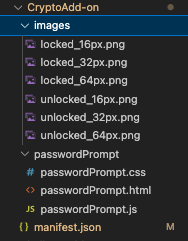
\includegraphics[width=0.6\textwidth]{fileStructureSoFar_1.png}
    \caption{\label{fig: folderStructure1} Development so far...}
\end{figure}



\subsection{Encrypt}
\subsection{Send message}



\chapter{Challenges Encountered}

\section{Open-source community}
\paragraph{Anything here?}

\section{Live development environment}
\paragraph{There were many challenge encountered, especially at the start. First, the author wanted to work through the four available Thunderbird add-on development tutorials. There was only one problem, after two simple "hello world" type tutorials, the last two did not work, as expected. A week or so of trying to figure it out -- far too long -- I finally asked for help. There were bugs! Thus, I became acquinted with the Mozilla bug tracker, \emph{Bugzilla}. Even though Thunderbird is considered to be an agnostic piece of software, that should work in Windows, Linux and Apple computer, it is not always the case. Apparently, development is chiefly done in Windows, and bugs for other systems are worked out over time. One of the most helpful developers, helpful to me on this journey, John Bieling, mentioned that he himself used Windows, and that he did not even have access to a Apple computer to debug some of the issues.}

\paragraph{My preferred platform is Apple OS, followed closely by Linux Mint. Lastly, if I have to, I will use Windows, which is what I had to use for this project. Even though sometimes during this process, I would revert to Apple or Linux platforms, ultimately, I came to the grim realization that it not advisable, because I could code something -- 100\% as it should be -- and it wouldn't work.}

\section{Nice to Haves - Backlog}
\paragraph{There were many areas where the developer failed, in one regard or another. In some cases, it was simply a juvenile and painful oversight at the start. There were many components that should have been included in the original specifications that the developer simply did not consider. This included common features of email clients that were completely overlooked:} 

\begin{enumerate}
\item Handle copying of emails to Sent folder
\end{enumerate}

\paragraph{If time allows, I will correct some of these elements.}

\paragraph{Which brings me to my second failure, of sorts. During the development process, I saw things that were not part of the original specifications, that could be considered "very nice to have" components. I could go back and change the specifications, and add these components -- and I will add them if \emph{time} allows. But, I want to stay genuine and committed to the specifications, and fulfill them before getting bogged down with "nice to have" features. For the time being the developer will add them to a backlog, and work on them up until the project is submitted, and thereafter, as ultimately, the project will serve not only as an academic exercise, but a development example by the author.}

\subsection{Backlog}
\paragraph{These are items that are being noted, that need to be added, improved or enhanced in the future:}

\begin{itemize}
\item Password Popup - Do not allow empty password
\item Password Popup - Deactivate "Encrypt" button, if password field empty
\end{itemize}

\chapter{Summary}

\section{Retrospective}

\paragraph{First, the developer has to acknowledge that \emph{now} he feels like he knows Mozilla's Thunderbird API. Additionally, the experience and knowledge in Javascript has expanded by leaps and bounds. So, professionally, the experience has been of significant importance for someone interesting in calling themselves a professional in internet technologies.}

\paragraph{This was the developer's very first full fledged project where he was not supported, by other more talented programmers. Additionally, it marked the first time that the developer worked in a real-time environment with other developers. I was not intimidated by this, at the time, because I did not know any better. Only later, when I saw developers arguing about something (stylistic), with one throwing down his "...in 40 years of software engineering experience" card, to which the respondent conceding defeat with his own "...that he only had 30+ years of software engineering experience" card. I knew then, I was swimming with the sharks. Fortunately, it came towards the end of my project.}

\paragraph{Regrettably, the implementation is not complete. It falls just short of meeting the specifications defined by the developer at the beginning, and further short of what should be expected in a complete turn-key solution. There were a number of things that the developer did not foresee before development began which, in itself, is a failing that inhibited a robust solution.}

\section{Next steps}

\paragraph{Nevertheless, the developer intends to smooth out the project, enhance shortcomings, and use it as an example of what the developer is fully capable of. The developer can take a break from academic writing, and just focus on hacking, debugging, testing, refining, and re-factoring.}

%%\chapter{Appendix}

\section{Specifications details}

% This tex file holds the personas png images made with another
% external website/program
\newpage
\subsection{Personas}

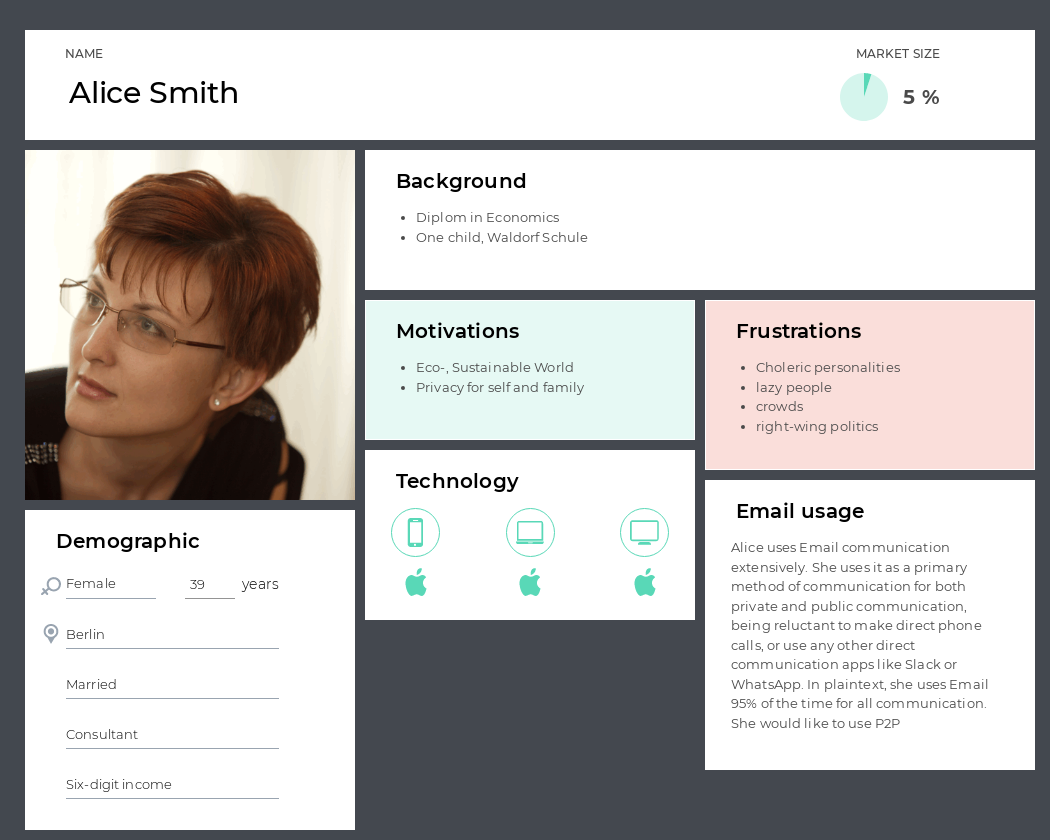
\includegraphics[scale=.38]{Alice Smith.png}
\\
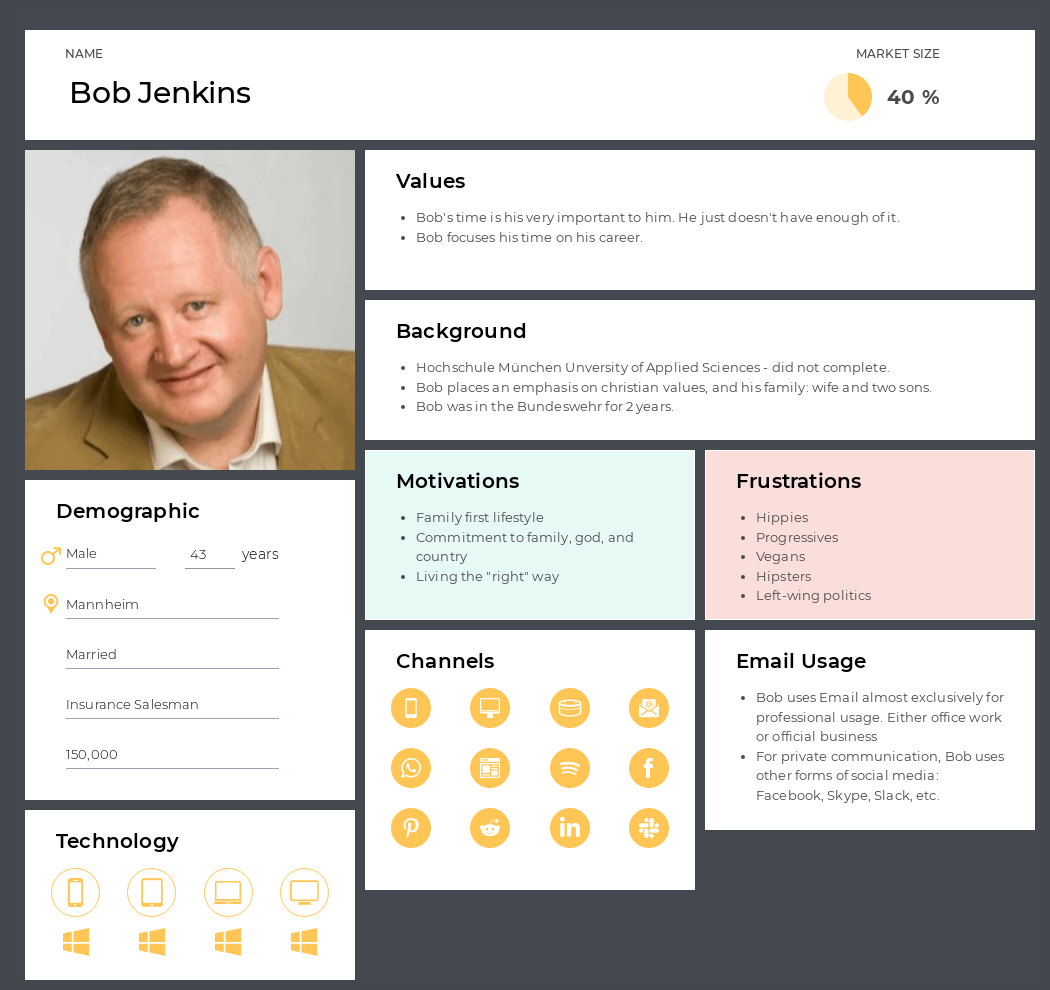
\includegraphics[scale=.38]{Bob Jenkins.png}

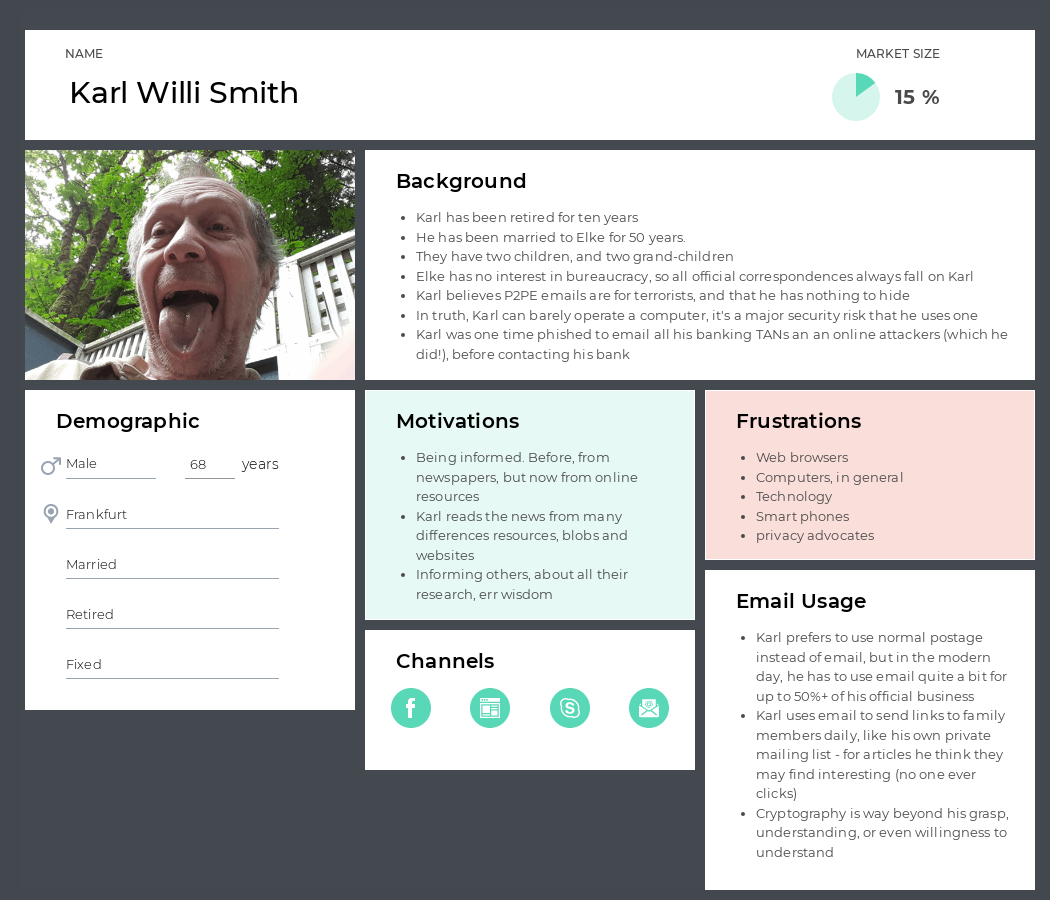
\includegraphics[scale=.38]{Karl Willi Smith.png}

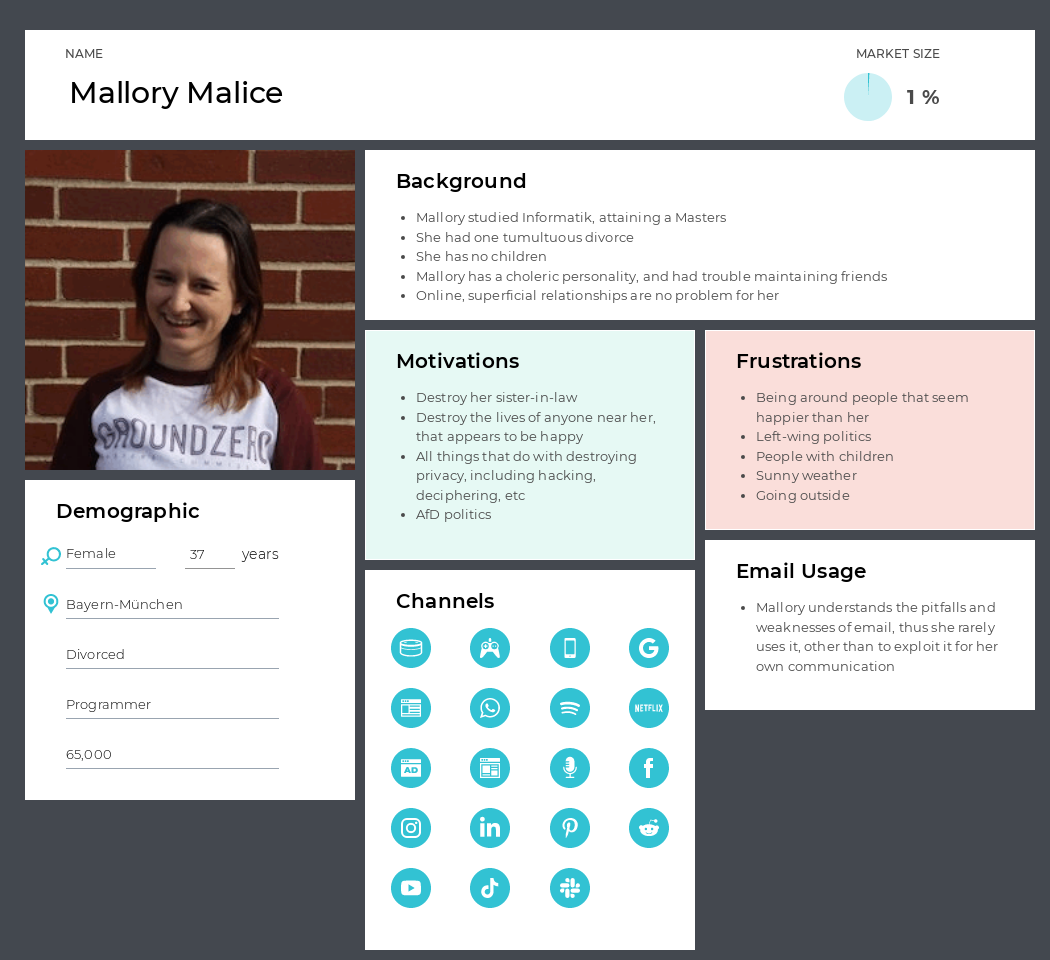
\includegraphics[scale=.38]{Mallory Malice.png}





%The following section will contain the 
\subsection{Use Cases}
\paragraph{The Use Cases used in this project will be defined, and or be restricted to the following items:}
\subsubsection{Use Case ID}
\paragraph{The Use Case ID will be a unique, numeric identifier for the use case.}

\subsubsection{Actor(s)}
\paragraph{An actor is a person or other entity external to the system who interacts with it, and performs use cases to complete task. Included in this designation, will be additional actors who participate in the use case.}

\subsubsection{Description}
\paragraph{This section should describe at a high level the purpose of the use case, what it aims to achieve, and any other relevant outcomes.}

\subsubsection{Preconditions}
\paragraph{The preconditions are all those conditions that must exist prior to the execution of the use case.}

\subsubsection{Basic Flow}
\paragraph{These are the basic, ordered steps and the description required for the completion of the use case. The steps will be numbers, and should be executed in this exact order. Completing the steps, in this order, should lead to the completion of the use case without error.}

\subsubsection{Exceptions}
\paragraph{Describes any anticipated errors that could occur during the execution of the use case, and how the system will handle these errors. The exceptions systems will not describe unanticipated errors, or error that are not included in the basic flow.}

\subsubsection{Postconditions}
\paragraph{Describes the state of all relevant parties, including the system, \emph{after} the execution of the use case.}
\newpage


\begin{longtable} {|p{3cm}|p{9cm}|} %[!htb]
%\begin{center}
%\resizebox {12cm}{!}{
%	\begin{tabular}{|p{2cm}|p{10cm}|}
	\hline
	%added the multicolumn command here to be able to make titles across different columns.
	%\multicolumn{2}{|c|}{Use Cases}\\ 
	%\hline
Use Case ID: & 0\\
	\hline
Actor(s): & Alice \\
	\hline
Description: & Alice will encrypt an email to Bob \\
	\hline
	\multicolumn{2}{|l|}{Preconditions:} \\
	\multicolumn{2}{|l|}{1. Thunderbird Email client installed.} \\
	\multicolumn{2}{|l|}{2. Thunderbird Email client configured to send and receive emails.}\\
	\multicolumn{2}{|l|}{3. Super-duper Addon installed.} \\
	\multicolumn{2}{|l|}{4. Email written} \\
	\hline
	\multicolumn{2}{|l|}{Basic Flow:} \\
	\multicolumn{2}{|l|}{1. Alice writes an email in Thunderbird.}\\
	\multicolumn{2}{|l|}{2. Alice locates and click on the add-on button.} \\
	\multicolumn{2}{|l|}{3. Observe: Alive sees a popup screen encrypt the email.} \\
	\multicolumn{2}{|l|}{4. Alice is prompted to enter a password.}\\
	\hline
	\hline
	\multicolumn{2}{|l|}{Exceptions:} \\
	\multicolumn{2}{|l|}{1. N/A} \\
%	\multicolumn{2}{|l|}{2.} \\
%	\multicolumn{2}{|l|}{3.} \\
%	\multicolumn{2}{|l|}{4.} \\
	\hline
	\hline
	\multicolumn{2}{|l|}{Postconditions:} \\
	\multicolumn{2}{|l|}{1. The email is enciphered.} \\
	\multicolumn{2}{|l|}{2. The addon window closes.} \\
	\multicolumn{2}{|l|}{3. Alice is returned to the Thunderbird client.} \\
	%\multicolumn{2}{|l|}{4.} \\
	\hline
\end{longtable}

%\begin{longtable} {|p{3cm}|p{9cm}|} %[!htb]
%%\begin{center}
%%\resizebox {12cm}{!}{
%%	\begin{tabular}{|p{2cm}|p{10cm}|}
%	\hline
%	%added the multicolumn command here to be able to make titles across different columns.
%	%\multicolumn{2}{|c|}{Use Cases}\\ 
%	%\hline
%Use Case ID: & 001\\
%	\hline
%Actor(s): & Alice Smith \\
%	\hline
%Description: & Alice cancels the processing of an email. \\
%	\hline
%	\multicolumn{2}{|l|}{Preconditions:} \\
%	\multicolumn{2}{|l|}{1. Thunderbird Email client installed.} \\
%	\multicolumn{2}{|l|}{2. Thunderbird Email client configured to send and receive emails.}\\
%	\multicolumn{2}{|l|}{3. Super-duper Add-on installed.} \\
%	\multicolumn{2}{|l|}{4. Email written} \\
%	\hline
%	\multicolumn{2}{|l|}{Basic Flow:} \\
%	\multicolumn{2}{|l|}{1. Alice writes an email in Thunderbird.}\\
%	\multicolumn{2}{|l|}{2. Alice locates and click on the Add-on button.} \\
%	\multicolumn{2}{|l|}{3. Observe: Alive sees a popup screen encrypt the email.} \\
%	\multicolumn{2}{|l|}{4. Alice is prompted to enter a password.}\\
%	\hline
%	\hline
%	\multicolumn{2}{|l|}{Exceptions:} \\
%	\multicolumn{2}{|l|}{1. Between every number option above, Alice can cancel the email.} \\
%%	\multicolumn{2}{|l|}{2.} \\
%%	\multicolumn{2}{|l|}{3.} \\
%%	\multicolumn{2}{|l|}{4.} \\
%	\hline
%	\hline
%	\multicolumn{2}{|l|}{Postconditions:} \\
%	\multicolumn{2}{|l|}{1. The email encryption is canceled.} \\
%	\multicolumn{2}{|l|}{2. The Add-on window closes.} \\
%	\multicolumn{2}{|l|}{3. Alice is returned to the Thunderbird client.} \\
%	%\multicolumn{2}{|l|}{4.} \\
%	\hline
%\end{longtable}

\begin{longtable} {|p{3cm}|p{9cm}|} %[!htb]
%\begin{center}
%\resizebox {12cm}{!}{
%	\begin{tabular}{|p{2cm}|p{10cm}|}
	\hline
	%added the multicolumn command here to be able to make titles across different columns.
	%\multicolumn{2}{|c|}{Use Cases}\\ 
	%\hline
Use Case ID: & 1\\
	\hline
Actor(s): & Bob (or any other intended recipient) decrypts an Email from Alice \\
	\hline
Description: & Alice will encrypt an email to another actor, then share a password with them, that they will then be able to decrypt \\
	\hline
	\multicolumn{2}{|l|}{Preconditions:} \\
	\multicolumn{2}{|l|}{1. Thunderbird Email client installed.} \\
	\multicolumn{2}{|l|}{2. Thunderbird Email client configured to send and receive emails.}\\
	\multicolumn{2}{|l|}{3. Super-duper Add-on installed.} \\
	\multicolumn{2}{|l|}{4. Email written} \\
	\hline
	\multicolumn{2}{|l|}{Basic Flow:} \\
	\multicolumn{2}{|l|}{1. Alice writes an email in Thunderbird.}\\
	\multicolumn{2}{|l|}{2. Alice locates and click on the addon button.} \\
	\multicolumn{2}{|l|}{3. Observe: Alive sees a popup screen encrypt the email.} \\
	\multicolumn{2}{|l|}{4. Alice is prompted to enter a password.}\\
	\multicolumn{2}{|l|}{5. Alice enters a password.} \\
	\multicolumn{2}{|l|}{4. Alice shares this password with said actor \emph{offline}.}\\
	\hline
	\hline
	\multicolumn{2}{|l|}{Exceptions:} \\
	\multicolumn{2}{|l|}{1. N/A} \\
%	\multicolumn{2}{|l|}{2.} \\
%	\multicolumn{2}{|l|}{3.} \\
%	\multicolumn{2}{|l|}{4.} \\
	\hline
	\hline
	\multicolumn{2}{|l|}{Postconditions:} \\
	\multicolumn{2}{|l|}{1. The email is enciphered.} \\
	\multicolumn{2}{|l|}{2. The addon window closes.} \\
	\multicolumn{2}{|l|}{3. Alice is returned to the Thunderbird client.} \\
	%\multicolumn{2}{|l|}{4.} \\
	\hline
\end{longtable}

%
%\begin{longtable} {|p{3cm}|p{9cm}|} %[!htb]
%%\begin{center}
%%\resizebox {12cm}{!}{
%%	\begin{tabular}{|p{2cm}|p{10cm}|}
%	\hline
%	%added the multicolumn command here to be able to make titles across different columns.
%	%\multicolumn{2}{|c|}{Use Cases}\\ 
%	%\hline
%Use Case ID: & 2\\
%	\hline
%Actor(s): & Bob (or any other intended recipient)\\
%	\hline
%Description: & Bob will decipher an email sent from Alice.\\
%	\hline
%	\multicolumn{2}{|l|}{Preconditions:} \\
%	\multicolumn{2}{|l|}{1. Thunderbird Email client installed.} \\
%	\multicolumn{2}{|l|}{2. Thunderbird Email client configured to send and receive emails.}\\
%	\multicolumn{2}{|l|}{3. Super-duper Add-on installed.} \\
%	\multicolumn{2}{|l|}{4. Enciphered Email received.} \\
%	\multicolumn{2}{|l|}{5. Deciphering password from Alice Smith received.} \\
%	\hline
%	\multicolumn{2}{|l|}{Basic Flow:} \\
%	\multicolumn{2}{|l|}{1. Bob opens his Thunderbird email client.}\\
%	\multicolumn{2}{|l|}{2. Bob notices an encrypted email from Alice in his inbox.} \\
%	\multicolumn{2}{|l|}{3. Bob selects the email.} \\
%	\multicolumn{2}{|l|}{3. Observe: A popup window appears, prompting Bob for a password.} \\
%	\multicolumn{2}{|l|}{4. Bob enters the password.}\\
%	\multicolumn{2}{|l|}{3. The email is deciphered, and can now be read.} \\
%	\hline
%	\hline
%	\multicolumn{2}{|l|}{Exceptions:} \\
%	\multicolumn{2}{|l|}{1. N/A} \\
%%	\multicolumn{2}{|l|}{2.} \\
%%	\multicolumn{2}{|l|}{3.} \\
%%	\multicolumn{2}{|l|}{4.} \\
%	\hline
%	\hline
%	\multicolumn{2}{|l|}{Postconditions:} \\
%	\multicolumn{2}{|l|}{1. The prompting window disappears.} \\
%	\multicolumn{2}{|l|}{2. The email can now be read..} \\
%%	\multicolumn{2}{|l|}{3. Alice is returned to the Thunderbird client.} \\
%	%\multicolumn{2}{|l|}{4.} \\
%	\hline
%\end{longtable}


%\begin{longtable} {|p{3cm}|p{9cm}|} %[!htb]
%\begin{center}
%\resizebox {12cm}{!}{
%	\begin{tabular}{|p{2cm}|p{10cm}|}
	%\hline
	%added the multicolumn command here to be able to make titles across different columns.
	%\multicolumn{2}{|c|}{Use Cases}\\ 
	%\hline
%Use Case ID: & 004\\
%	\hline
%Actor(s): & Alice Smith \\
%	\hline
%Description: & Alice will encrypt an email to Bob \\
%	\hline
%	\multicolumn{2}{|l|}{Preconditions:} \\
%	\multicolumn{2}{|l|}{1. Thunderbird Email client installed.} \\
%	\multicolumn{2}{|l|}{2. Thunderbird Email client configured to send and receive emails.}\\
%	\multicolumn{2}{|l|}{3. Super-duper Addon installed.} \\
%	\multicolumn{2}{|l|}{4. Email written} \\
%	\hline
%	\multicolumn{2}{|l|}{Basic Flow:} \\
%	\multicolumn{2}{|l|}{1. Alice writes an email in Thunderbird.}\\
%	\multicolumn{2}{|l|}{2. Alice locates and click on the addon button.} \\
%	\multicolumn{2}{|l|}{3. Observe: Alive sees a popup screen encrypt the email.} \\
%	\multicolumn{2}{|l|}{4. Alice is prompted to enter a password.}\\
%	\hline
%	\hline
%	\multicolumn{2}{|l|}{Exceptions:} \\
%	\multicolumn{2}{|l|}{1. None allowed. =)} \\
%%	\multicolumn{2}{|l|}{2.} \\
%%	\multicolumn{2}{|l|}{3.} \\
%%	\multicolumn{2}{|l|}{4.} \\
%	\hline
%	\hline
%	\multicolumn{2}{|l|}{Postconditions:} \\
%	\multicolumn{2}{|l|}{1. The email is enciphered.} \\
%	\multicolumn{2}{|l|}{2. The addon window closes.} \\
%	\multicolumn{2}{|l|}{3. Alice is returned to the Thunderbird client.} \\
%	%\multicolumn{2}{|l|}{4.} \\
%	\hline
%\end{longtable}
%
%
%\begin{longtable} {|p{3cm}|p{9cm}|} %[!htb]
%%\begin{center}
%%\resizebox {12cm}{!}{
%%	\begin{tabular}{|p{2cm}|p{10cm}|}
%	\hline
%	%added the multicolumn command here to be able to make titles across different columns.
%	%\multicolumn{2}{|c|}{Use Cases}\\ 
%	%\hline
%Use Case ID: & 005\\
%	\hline
%Actor(s): & Alice Smith \\
%	\hline
%Description: & Alice will encrypt an email to Bob \\
%	\hline
%	\multicolumn{2}{|l|}{Preconditions:} \\
%	\multicolumn{2}{|l|}{1. Thunderbird Email client installed.} \\
%	\multicolumn{2}{|l|}{2. Thunderbird Email client configured to send and receive emails.}\\
%	\multicolumn{2}{|l|}{3. Super-duper Addon installed.} \\
%	\multicolumn{2}{|l|}{4. Email written} \\
%	\hline
%	\multicolumn{2}{|l|}{Basic Flow:} \\
%	\multicolumn{2}{|l|}{1. Alice writes an email in Thunderbird.}\\
%	\multicolumn{2}{|l|}{2. Alice locates and click on the addon button.} \\
%	\multicolumn{2}{|l|}{3. Observe: Alive sees a popup screen encrypt the email.} \\
%	\multicolumn{2}{|l|}{4. Alice is prompted to enter a password.}\\
%	\hline
%	\hline
%	\multicolumn{2}{|l|}{Exceptions:} \\
%	\multicolumn{2}{|l|}{1. None allowed. =)} \\
%%	\multicolumn{2}{|l|}{2.} \\
%%	\multicolumn{2}{|l|}{3.} \\
%%	\multicolumn{2}{|l|}{4.} \\
%	\hline
%	\hline
%	\multicolumn{2}{|l|}{Postconditions:} \\
%	\multicolumn{2}{|l|}{1. The email is enciphered.} \\
%	\multicolumn{2}{|l|}{2. The addon window closes.} \\
%	\multicolumn{2}{|l|}{3. Alice is returned to the Thunderbird client.} \\
%	%\multicolumn{2}{|l|}{4.} \\
%	\hline
%\end{longtable}
%
%
%\begin{longtable} {|p{3cm}|p{9cm}|} %[!htb]
%%\begin{center}
%%\resizebox {12cm}{!}{
%%	\begin{tabular}{|p{2cm}|p{10cm}|}
%	\hline
%	%added the multicolumn command here to be able to make titles across different columns.
%	%\multicolumn{2}{|c|}{Use Cases}\\ 
%	%\hline
%Use Case ID: & 006\\
%	\hline
%Actor(s): & Alice Smith \\
%	\hline
%Description: & Alice will encrypt an email to Bob \\
%	\hline
%	\multicolumn{2}{|l|}{Preconditions:} \\
%	\multicolumn{2}{|l|}{1. Thunderbird Email client installed.} \\
%	\multicolumn{2}{|l|}{2. Thunderbird Email client configured to send and receive emails.}\\
%	\multicolumn{2}{|l|}{3. Super-duper Addon installed.} \\
%	\multicolumn{2}{|l|}{4. Email written} \\
%	\hline
%	\multicolumn{2}{|l|}{Basic Flow:} \\
%	\multicolumn{2}{|l|}{1. Alice writes an email in Thunderbird.}\\
%	\multicolumn{2}{|l|}{2. Alice locates and click on the addon button.} \\
%	\multicolumn{2}{|l|}{3. Observe: Alive sees a popup screen encrypt the email.} \\
%	\multicolumn{2}{|l|}{4. Alice is prompted to enter a password.}\\
%	\hline
%	\hline
%	\multicolumn{2}{|l|}{Exceptions:} \\
%	\multicolumn{2}{|l|}{1. None allowed. =)} \\
%%	\multicolumn{2}{|l|}{2.} \\
%%	\multicolumn{2}{|l|}{3.} \\
%%	\multicolumn{2}{|l|}{4.} \\
%	\hline
%	\hline
%	\multicolumn{2}{|l|}{Postconditions:} \\
%	\multicolumn{2}{|l|}{1. The email is enciphered.} \\
%	\multicolumn{2}{|l|}{2. The addon window closes.} \\
%	\multicolumn{2}{|l|}{3. Alice is returned to the Thunderbird client.} \\
%	%\multicolumn{2}{|l|}{4.} \\
%	\hline
%\end{longtable}
%
%
%\begin{longtable} {|p{3cm}|p{9cm}|} %[!htb]
%%\begin{center}
%%\resizebox {12cm}{!}{
%%	\begin{tabular}{|p{2cm}|p{10cm}|}
%	\hline
%	%added the multicolumn command here to be able to make titles across different columns.
%	%\multicolumn{2}{|c|}{Use Cases}\\ 
%	%\hline
%Use Case ID: & 007\\
%	\hline
%Actor(s): & Alice Smith \\
%	\hline
%Description: & Alice will encrypt an email to Bob \\
%	\hline
%	\multicolumn{2}{|l|}{Preconditions:} \\
%	\multicolumn{2}{|l|}{1. Thunderbird Email client installed.} \\
%	\multicolumn{2}{|l|}{2. Thunderbird Email client configured to send and receive emails.}\\
%	\multicolumn{2}{|l|}{3. Super-duper Addon installed.} \\
%	\multicolumn{2}{|l|}{4. Email written} \\
%	\hline
%	\multicolumn{2}{|l|}{Basic Flow:} \\
%	\multicolumn{2}{|l|}{1. Alice writes an email in Thunderbird.}\\
%	\multicolumn{2}{|l|}{2. Alice locates and click on the addon button.} \\
%	\multicolumn{2}{|l|}{3. Observe: Alive sees a popup screen encrypt the email.} \\
%	\multicolumn{2}{|l|}{4. Alice is prompted to enter a password.}\\
%	\hline
%	\hline
%	\multicolumn{2}{|l|}{Exceptions:} \\
%	\multicolumn{2}{|l|}{1. None allowed. =)} \\
%%	\multicolumn{2}{|l|}{2.} \\
%%	\multicolumn{2}{|l|}{3.} \\
%%	\multicolumn{2}{|l|}{4.} \\
%	\hline
%	\hline
%	\multicolumn{2}{|l|}{Postconditions:} \\
%	\multicolumn{2}{|l|}{1. The email is enciphered.} \\
%	\multicolumn{2}{|l|}{2. The addon window closes.} \\
%	\multicolumn{2}{|l|}{3. Alice is returned to the Thunderbird client.} \\
%	%\multicolumn{2}{|l|}{4.} \\
%	\hline
%\end{longtable}
%
%\begin{longtable} {|p{3cm}|p{9cm}|} %[!htb]
%%\begin{center}
%%\resizebox {12cm}{!}{
%%	\begin{tabular}{|p{2cm}|p{10cm}|}
%	\hline
%	%added the multicolumn command here to be able to make titles across different columns.
%	%\multicolumn{2}{|c|}{Use Cases}\\ 
%	%\hline
%Use Case ID: & 008\\
%	\hline
%Actor(s): & Alice Smith \\
%	\hline
%Description: & Alice will encrypt an email to Bob \\
%	\hline
%	\multicolumn{2}{|l|}{Preconditions:} \\
%	\multicolumn{2}{|l|}{1. Thunderbird Email client installed.} \\
%	\multicolumn{2}{|l|}{2. Thunderbird Email client configured to send and receive emails.}\\
%	\multicolumn{2}{|l|}{3. Super-duper Addon installed.} \\
%	\multicolumn{2}{|l|}{4. Email written} \\
%	\hline
%	\multicolumn{2}{|l|}{Basic Flow:} \\
%	\multicolumn{2}{|l|}{1. Alice writes an email in Thunderbird.}\\
%	\multicolumn{2}{|l|}{2. Alice locates and click on the addon button.} \\
%	\multicolumn{2}{|l|}{3. Observe: Alive sees a popup screen encrypt the email.} \\
%	\multicolumn{2}{|l|}{4. Alice is prompted to enter a password.}\\
%	\hline
%	\hline
%	\multicolumn{2}{|l|}{Exceptions:} \\
%	\multicolumn{2}{|l|}{1. None allowed. =)} \\
%%	\multicolumn{2}{|l|}{2.} \\
%%	\multicolumn{2}{|l|}{3.} \\
%%	\multicolumn{2}{|l|}{4.} \\
%	\hline
%	\hline
%	\multicolumn{2}{|l|}{Postconditions:} \\
%	\multicolumn{2}{|l|}{1. The email is enciphered.} \\
%	\multicolumn{2}{|l|}{2. The addon window closes.} \\
%	\multicolumn{2}{|l|}{3. Alice is returned to the Thunderbird client.} \\
%	%\multicolumn{2}{|l|}{4.} \\
%	\hline
%\end{longtable}
%
%\begin{longtable} {|p{3cm}|p{9cm}|} %[!htb]
%%\begin{center}
%%\resizebox {12cm}{!}{
%%	\begin{tabular}{|p{2cm}|p{10cm}|}
%	\hline
%	%added the multicolumn command here to be able to make titles across different columns.
%	%\multicolumn{2}{|c|}{Use Cases}\\ 
%	%\hline
%Use Case ID: & 009\\
%	\hline
%Actor(s): & Alice Smith \\
%	\hline
%Description: & Alice will encrypt an email to Bob \\
%	\hline
%	\multicolumn{2}{|l|}{Preconditions:} \\
%	\multicolumn{2}{|l|}{1. Thunderbird Email client installed.} \\
%	\multicolumn{2}{|l|}{2. Thunderbird Email client configured to send and receive emails.}\\
%	\multicolumn{2}{|l|}{3. Super-duper Addon installed.} \\
%	\multicolumn{2}{|l|}{4. Email written} \\
%	\hline
%	\multicolumn{2}{|l|}{Basic Flow:} \\
%	\multicolumn{2}{|l|}{1. Alice writes an email in Thunderbird.}\\
%	\multicolumn{2}{|l|}{2. Alice locates and click on the addon button.} \\
%	\multicolumn{2}{|l|}{3. Observe: Alive sees a popup screen encrypt the email.} \\
%	\multicolumn{2}{|l|}{4. Alice is prompted to enter a password.}\\
%	\hline
%	\hline
%	\multicolumn{2}{|l|}{Exceptions:} \\
%	\multicolumn{2}{|l|}{1. None allowed. =)} \\
%%	\multicolumn{2}{|l|}{2.} \\
%%	\multicolumn{2}{|l|}{3.} \\
%%	\multicolumn{2}{|l|}{4.} \\
%	\hline
%	\hline
%	\multicolumn{2}{|l|}{Postconditions:} \\
%	\multicolumn{2}{|l|}{1. The email is enciphered.} \\
%	\multicolumn{2}{|l|}{2. The addon window closes.} \\
%	\multicolumn{2}{|l|}{3. Alice is returned to the Thunderbird client.} \\
%	%\multicolumn{2}{|l|}{4.} \\
%	\hline
%\end{longtable}
%
\begin{longtable} {|p{3cm}|p{9cm}|} %[!htb]
%\begin{center}
%\resizebox {12cm}{!}{
%	\begin{tabular}{|p{2cm}|p{10cm}|}
	\hline
	%added the multicolumn command here to be able to make titles across different columns.
	%\multicolumn{2}{|c|}{Use Cases}\\ 
	%\hline
Use Case ID: & 2\\
	\hline
Actor(s): & Mallory \\
	\hline
Description: & Mallory will decipher an email \\
	\hline
	\multicolumn{2}{|l|}{Preconditions:} \\
	\multicolumn{2}{|l|}{1. Thunderbird Email client installed.} \\
	\multicolumn{2}{|l|}{2. Thunderbird Email client configured to send and receive emails.}\\
	\multicolumn{2}{|l|}{3. Super-duper Addon installed.} \\
	\multicolumn{2}{|l|}{4. Email written} \\
	\hline
	\multicolumn{2}{|l|}{Basic Flow:} \\
	\multicolumn{2}{|l|}{1. Alice writes an email in Thunderbird.}\\
	\multicolumn{2}{|l|}{2. Alice locates and click on the addon button.} \\
	\multicolumn{2}{|l|}{3. Observe: Alive sees a popup screen encrypt the email.} \\
	\multicolumn{2}{|l|}{4. Alice is prompted to enter a password.}\\
	\multicolumn{2}{|l|}{5. TBD.}\\
	\hline
	\hline
	\multicolumn{2}{|l|}{Exceptions:} \\
	\multicolumn{2}{|l|}{1. None allowed. =)} \\
%	\multicolumn{2}{|l|}{2.} \\
%	\multicolumn{2}{|l|}{3.} \\
%	\multicolumn{2}{|l|}{4.} \\
	\hline
	\hline
	\multicolumn{2}{|l|}{Postconditions:} \\
	\multicolumn{2}{|l|}{1. The email is still enciphered.} \\
	\multicolumn{2}{|l|}{2. The add-on window closes.} \\
	\multicolumn{2}{|l|}{3. Mallory is returned to the Thunderbird client.} \\
	%\multicolumn{2}{|l|}{4.} \\
	\hline
\end{longtable}

\subsection{Use Case Diagrams}

\section{Software Requirements}

%This template was made by Drexl Spivey
%It is a derived from the IEEE Standard 830-1998 for writing
%Software Requirements Specifications

\chapter{Software Requirements Specifications}
\section{Introduction}
%The introduction of the SRS should provide an overview of the entire SRS. It should contain the following
%subsections:
%a) Purpose;
%b) Scope;
%c) Definitions, acronyms, and abbreviations;
%d) References;
%e) Overview.

\subsection{Purpose}
%This subsection should
%a) Delineate the purpose of the SRS;
%b) Specify the intended audience for the SRS.
\paragraph{This document will describe the entire software development process, including use cases, personas, diagrams, and the end goals of the system. The audience for this document will be any persons interested in the software engineering process used for this project, but more specifically, those responsible for overseeing and rating this project.}



\subsection{Scope}
%This subsection should
%a) Identify the software product(s) to be produced by name (e.g., Host DBMS, Report Generator, etc.);
%b) Explain what the software product(s) will, and, if necessary, will not do;
%c) Describe the application of the software being specified, including relevant benefits, objectives, and goals;
%d) Be consistent with similar statements in higher-level specifications (e.g., the system requirements specification), if they exist.
\paragraph{The name for this product will be "Thunderbird: One Time Password." This product will be a Thunderbird add-on, that will encipher plain text into cipher text, which will be delivered by the Thunderbird client to another Thunderbird recipient, that also has the add-on installed. Finally, the second person will be able to decipher the cipher text back to plain text, and read the message.}

\subsection{Definitions, acronyms, abbreviations}
%This subsection should provide the definitions of all terms, acronyms, and abbreviations required to properly interpret the SRS. This information may be provided by reference to one or more appendixes in the SRS or by reference to other documents.
\paragraph{The following definitions, acronyms, and abbreviations may be used with in the software development process:}

\begin{description}[font=\sffamily\bfseries, leftmargin=1cm]
\item[AES] Advanced Encryption Standard.
\item[API] application programming interface.
\item[asymmetric encryption] Encryption that requires two keys, one on each side of the private message exchange.
\item[CBC] Cipher Block Chaining, a AES encryption mode.
\item[CFB] Cipher Feedback Mode, a AES encryption mode.
\item[cipher text] The encrypted text.
\item[client] Refers to an email client, more specifically Mozilla's Thunderbird email client.
\item[CTR] Counter Mode, a AES encryption mode.
\item[E2EE] End-to-end encrypted, in this case, an end-to-end encrypted email.
\item[ECB] Electronic Codebook, a AES encryption mode.
\item[extensions] An extension adds features and functions to a browser.
\item[IEEE] Institute of Electrical and Electronics Engineers.
\item[JS] JavaScript.
\item[OFB] Output Feedback Mode, a AES encryption mode.
\item[plain text] The text that we wish to encrypt.
\item[SRS] Software Requirements Specification.
\item[symmetric encryption] Encryption that only uses one key for encryption.
\end{description}

\subsection{Software Requirements References}
%This subsection should
%a) Provide a complete list of all documents referenced elsewhere in the SRS;
%b) Identify each document by title, report number (if applicable), date, and publishing organization;
%c) Specify the sources from which the references can be obtained.
%
%This information may be provided by reference to an appendix or to another document
\paragraph{Author used the IEEE document:}
\begin{enumerate}
\item IEEE Std 803-1998
\end{enumerate}
\paragraph{the IEEE Recommended Practice for Software Requirements Specifications.}\footnote{https://cse.msu.edu/~cse870/IEEEXplore-SRS-template.pdf}

%\subsection{Overview}
%This subsection should
%a) Describe what the rest of the SRS contains;
%b) Explain how the SRS is organized.

\section{Overall Description}
%This section of the SRS should describe the general factors that affect the product and its requirements. This
%section does not state specific requirements. Instead, it provides a background for those requirements, which
%are defined in detail in Section 3 of the SRS, and makes them easier to understand.
%This section usually consists of six subsections, as follows:
%a) Product perspective;
%b) Product functions;
%c) User characteristics;
%d) Constraints;
%e) Assumptions and dependencies;
%f) Apportioning of requirements.
\paragraph{The following subsections will describe the general factors that will influence the product requirements, including any background information.}
 
\subsection{Product perspective}
%This subsection of the SRS should put the product into perspective with other related products. If the product is independent and totally self-contained, it should be so stated here. If the SRS defines a product that is a component of a larger system, as frequently occurs, then this subsection should relate the requirements of that larger system to functionality of the software and should identify interfaces between that system and the software.
%
%A block diagram showing the major components of the larger system, interconnections, and external inter-
%faces can be helpful.
%
%This subsection should also describe how the software operates inside various constraints. For example,
%these constraints could include
%a) System interfaces;
%b) User interfaces;
%c) Hardware interfaces;
%d) Software interfaces;
%e) Communications interfaces;
%f) Memory;
%g) Operations;
%h) Site adaptation requirements.
\paragraph{The developed software product, \emph{Thunderbird: One Time Password}, has not current rival. It current alternatives would be Mozilla's own implementation of OpenPGP. The previous option was PGP through the add-on Enigmail. However, at the writing of this document, the add-on is no longer supported.}
\paragraph{The two alternatives to this proposal do have the advantage that they use asymmetric key exchange to encrypt emails, which is more secure, and recommended for encoded email exchange. The \emph{Thunderbird: One Time Password} add-on will have the feature that it is easy to use, at the expense of some security.}


\subsubsection{System interfaces}
%This should list each system interface and identify the functionality of the software to accomplish the system requirement and the interface description to match the system.
\paragraph{The interfaces required for the product include the following:}
\begin{enumerate}
\item A modern system, running one of three operating systems:
\begin{enumerate}
\item Windows 10 or later
\item Apple running Big Sur or later
\item Linux variant like Debian 10+ or Mint 21+
\end{enumerate}
\item an Internet connection
\end{enumerate}


\subsubsection{User interfaces}
%This should specify the following:
%a) The logical characteristics of each interface between the software product and its users. This
%includes those configuration characteristics (e.g., required screen formats, page or window layouts,
%content of any reports or menus, or availability of programmable function keys) necessary to accomplish the software requirements.
%b) All the aspects of optimizing the interface with the person who must use the system. This may simply
%comprise a list of do's and dont's on how the system will appear to the user. One example may be a
%requirement for the option of long or short error messages. Like all others, these requirements
%should be verifiable, e.g., a clerk typist grade 4 can do function X in Z min after 1 h of training
%rather than a typist can do function X. (This may also be specified in the Software System
%Attributes under a section titled Ease of Use.)
\paragraph{There are no special user interface requirements.}

\subsubsection{Hardware interfaces}
%This should specify the logical characteristics of each interface between the software product and the hardware components of the system. This includes configuration characteristics (number of ports, instruction sets, etc.). It also covers such matters as what devices are to be supported, how they are to be supported, and protocols. For example, terminal support may specify full-screen support as opposed to line-by-line support.
\paragraph{There are no special hardware interfaces required for this product to function.}

\subsubsection{Software interfaces}
%This should specify the use of other required software products (e.g., a data management system, an operating system, or a mathematical package), and interfaces with other application systems (e.g., the linkage between an accounts receivable system and a general ledger system). For each required software product, the following should be provided:
%
%\begin{enumerate}
%\item Name
%\item Mnemonic
%\item Specification number
%\item Version number
%\item Source
%\end{enumerate}
%
%For each interface, the following should be provided:
%\begin{enumerate}
%\item Discussion of the purpose of the interfacing software as related to this software product.
%\item Definition of the interface in terms of message content and format. It is not necessary to detail any well-documented interface, but a reference to the document defining the interface is required.
%\end{enumerate}

\paragraph{The required software interfaces are:}
\begin{enumerate}
\item Mozilla's free, open source email client, Thunderbird, to be installed on the system.
\item The client should be configured to send and receive emails.\footnote{Thus, an email account on an email server is assumed.}
\item The client should be updated to the latest current software version.
\item The client can be installed and tested on Windows 10, Linux Cinnamon Mind 21, and macOS Monterey.
\end{enumerate}



\subsubsection{Communications interfaces}
%This should specify the various interfaces to communications such as local network protocols, etc.
\paragraph{No special communication interfaces will be required, than would already be prerequisites for email communication, i.e. network capable computer.}

\subsubsection{Memory constraints}
%This should specify any applicable characteristics and limits on primary and secondary memory.
\paragraph{Not applicable}


\subsubsection{Operations}
%This should specify the normal and special operations required by the user such as
%a) The various modes of operations in the user organization (e.g., user-initiated operations);
%b) Periods of interactive operations and periods of unattended operations;
%c) Data processing support functions; 
%d) Backup and recovery operations.
%
%NOTE - This is sometimes specified as part of the User Interfaces section.
\paragraph{Not applicable}

\subsubsection{Site adaptation requirements}
%This should
%a) Define the requirements for any data or initialization sequences that are specific to a given site,
%mission, or operational mode (e.g., grid values, safety limits, etc.);
%b) Specify the site or mission-related features that should be modified to adapt the software to a particular installation.
\paragraph{Not applicable}






%\subsection{Product functions}
%This subsection of the SRS should provide a summary of the major functions that the software will perform.
%For example, an SRS for an accounting program may use this part to address customer account maintenance,
%customer statement, and invoice preparation without mentioning the vast amount of detail that each of those functions requires.
%Sometimes the function summary that is necessary for this part can be taken directly from the section of the higher-level specification (if one exists) that allocates particular functions to the software product. Note that for the sake of clarity
%a) The functions should be organized in a way that makes the list of functions understandable to the
%customer or to anyone else reading the document for the first time.
%b) Textual or graphical methods can be used to show the different functions and their relationships.
%Such a diagram is not intended to show a design of a product, but simply shows the logical relation-
%ships among variables.




\subsection{User characteristics}
%This subsection of the SRS should describe those general characteristics of the intended users of the product including educational level, experience, and technical expertise. It should not be used to state specific requirements, but rather should provide the reasons why certain specific requirements are later specified in Section 3 of the SRS.
\paragraph{See Personas in the appendix.}

\subsection{Constraints}
%This subsection of the SRS should provide a general description of any other items that will limit the developer's options. These include:
%a) Regulatory policies;
%b) Hardware limitations (e.g., signal timing requirements);
%c) Interfaces to other applications;
%d) Parallel operation;
%e) Audit functions;
%f) Control functions;
%g) Higher-order language requirements;
%h) Signal handshake protocols (e.g., XON-XOFF, ACK-NACK);
%i) Reliability requirements;
%j) Criticality of the application;
%k) Safety and security considerations.
\paragraph{There will be various constraints within this project listed below:}
\begin{itemize}
\item Security: It will not be possible to account for all attack vectors. Thus, they will not be explored at this time.
%\item Security: How Mallory comes into possession of an encrypted email may not be fully explored. Related to 1. above, but we'll at least give an examination to this possibility -- however she came into possess the email.
\end{itemize}


%\subsection{Assumptions and dependencies}
%This subsection of the SRS should list each of the factors that affect the requirements stated in the SRS.
%These factors are not design constraints on the software but are, rather, any changes to them that can affect the requirements in the SRS. For example, an assumption may be that a specific operating system will be available on the hardware designated for the software product. If, in fact, the operating system is not available, the SRS would then have to change accordingly.

% Not sure what to do with this??
%5.2.6 Apportioning of requirements (2.6 of the SRS)
%This subsection of the SRS should identify requirements that may be delayed until future versions of the
%system.

\section{Specific Requirements}
%This section of the SRS should contain all of the software requirements to a level of detail sufficient to
%enable designers to design a system to satisfy those requirements, and testers to test that the system satisfies those requirements. Throughout this section, every stated requirement should be externally perceivable by users, operators, or other external systems. These requirements should include at a minimum a description of every input (stimulus) into the system, every output (response) from the system, and all functions performed by the system in response to an input or in support of an output. As this is often the largest and most important part of the SRS, the following principles apply:
%a) Specific requirements should be stated in conformance with all the characteristics described in 4.3.
%b) Specific requirements should be cross-referenced to earlier documents that relate.
%c) All requirements should be uniquely identifiable.
%d) Careful attention should be given to organizing the requirements to maximize readability.

%Before examining specific ways of organizing the requirements it is helpful to understand the various items that comprise requirements as described in 5.3.1 through 5.3.7.

\input{UseCaseTemplate}

%% Use Case Diagrams

%TODO These are pretty junk - fix or remove later

\subsection{Use Case Diagrams}

%\begin{wrapfigure}{R}{0.3\textwidth}
%\begin{center}
%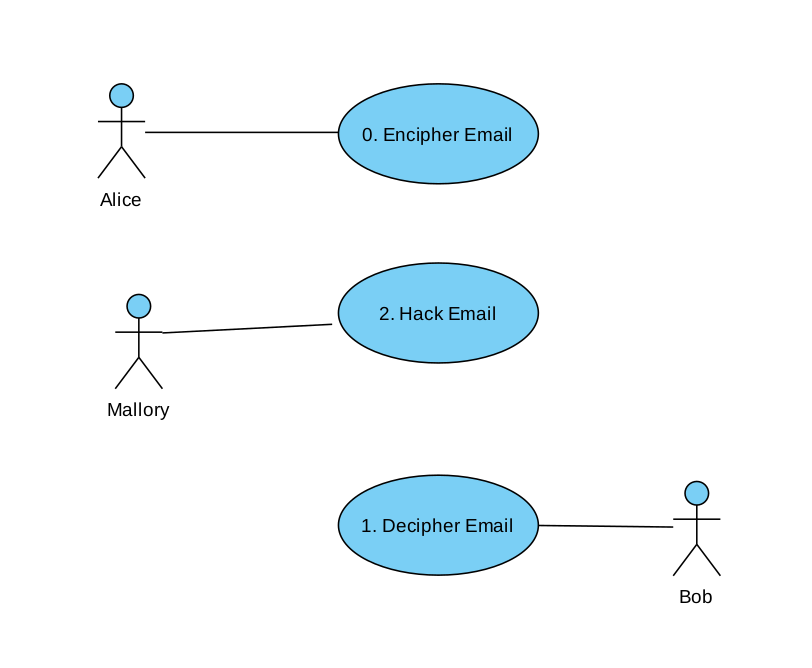
\includegraphics[scale=.50]{useCaseDiagram.png}
%\end{center}
%\end{wrapfigure}

\begin{figure}
    \centering
    \textbf{Use Case Diagrams}\par\medskip
    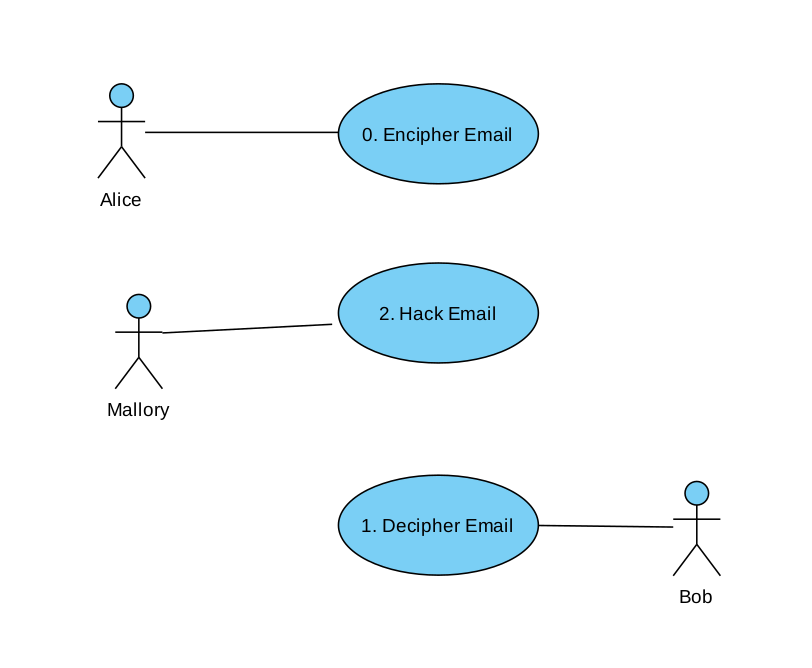
\includegraphics[scale=0.5]{useCaseDiagram.png}
%    \caption{Your caption}
\end{figure}

%\section{Appendix}
%The appendixes are not always considered part of the actual SRS and are not always necessary. They may
%include
%a) Sample input/output formats, descriptions of cost analysis studies, or results of user surveys;
%b) Supporting or background information that can help the readers of the SRS;
%c) A description of the problems to be solved by the software;
%d) Special packaging instructions for the code and the media to meet security, export, initial loading, or
%other requirements.
%
%When appendixes are included, the SRS should explicitly state whether or not the appendixes are to be
%considered part of the requirements.


%%These were added in this particular project.
% This tex file holds the personas png images made with another
% external website/program
\newpage
\subsection{Personas}

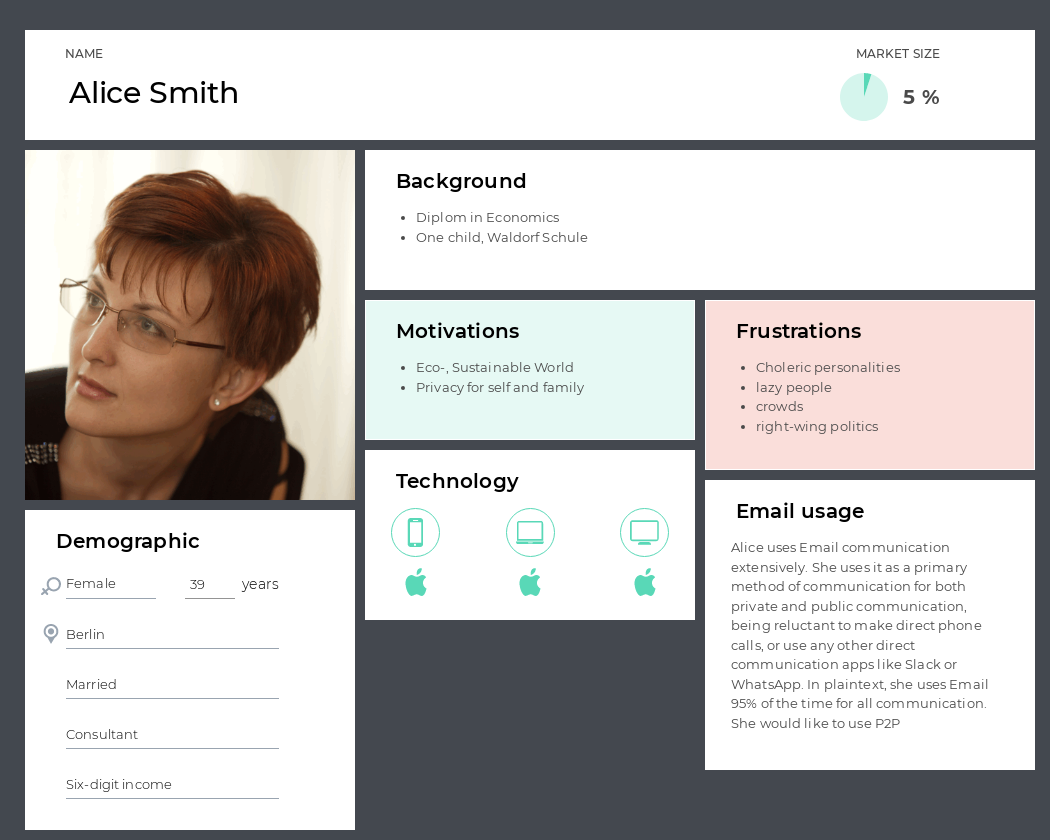
\includegraphics[scale=.38]{Alice Smith.png}
\\
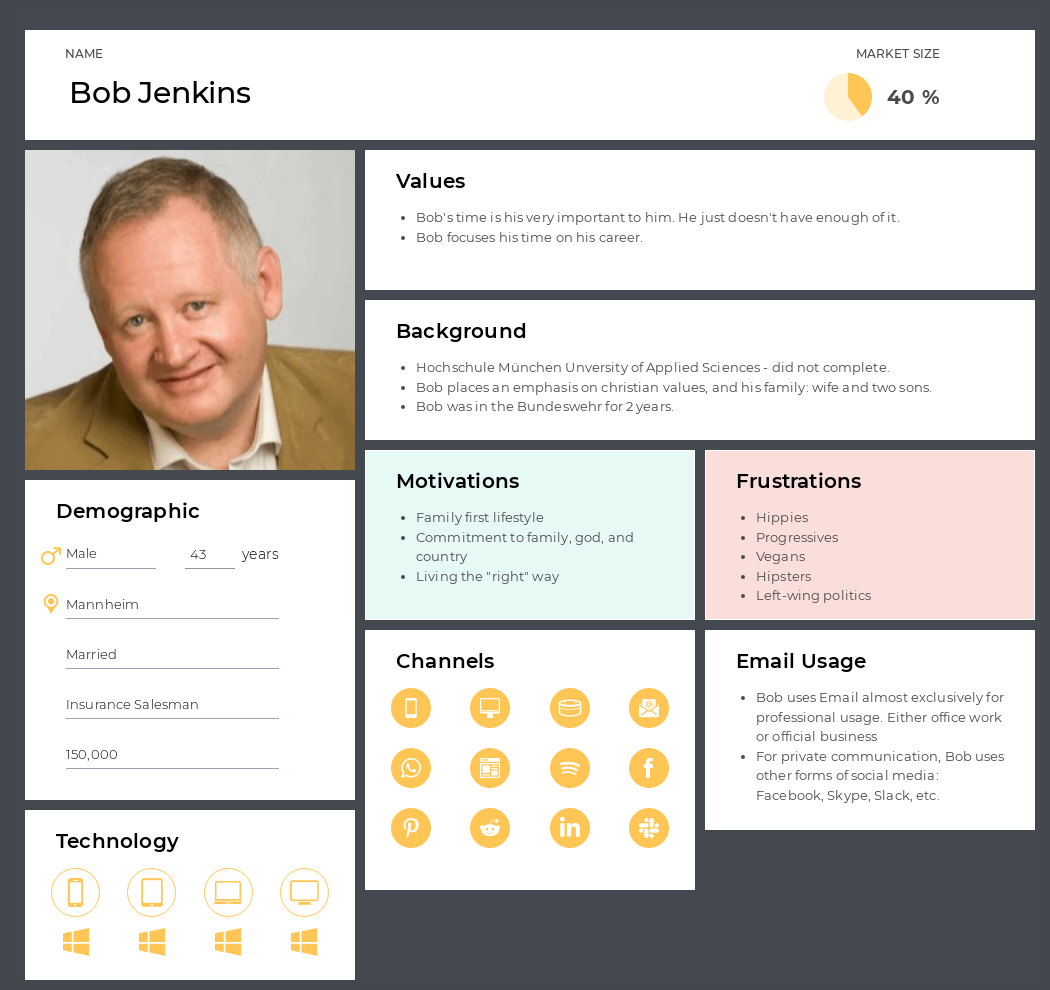
\includegraphics[scale=.38]{Bob Jenkins.png}

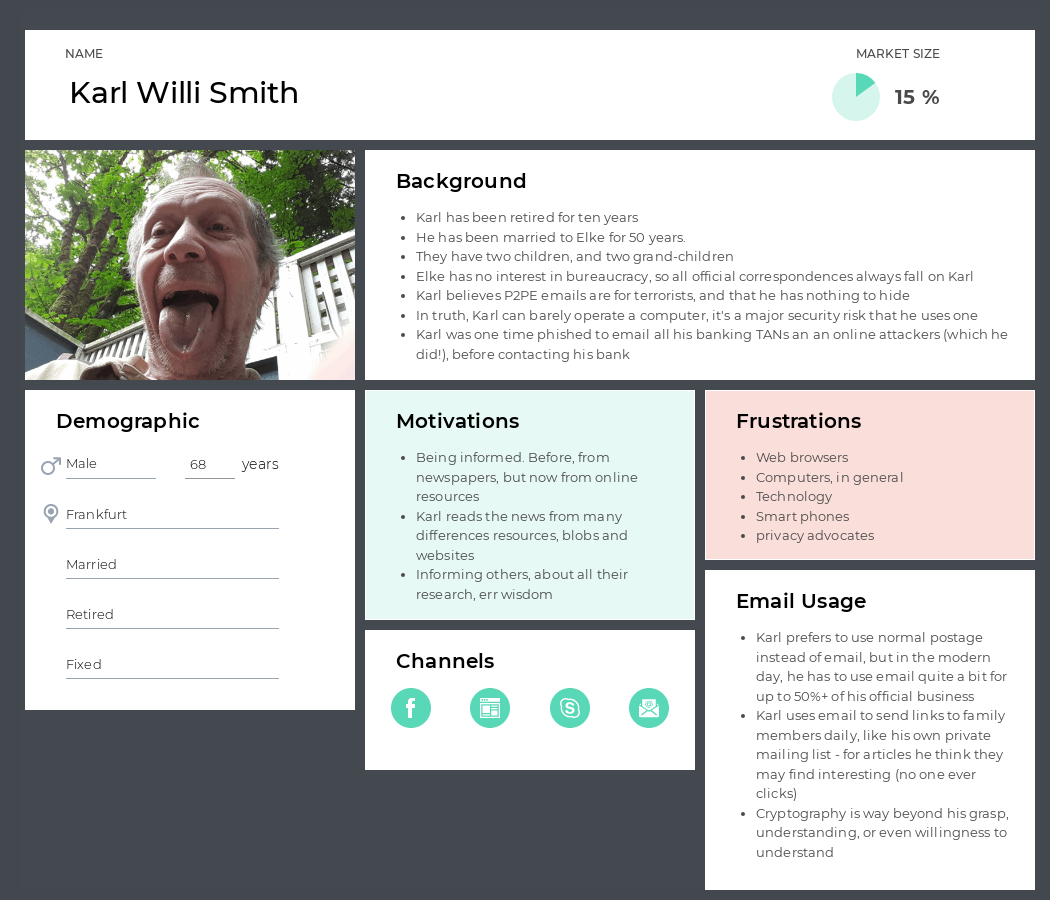
\includegraphics[scale=.38]{Karl Willi Smith.png}

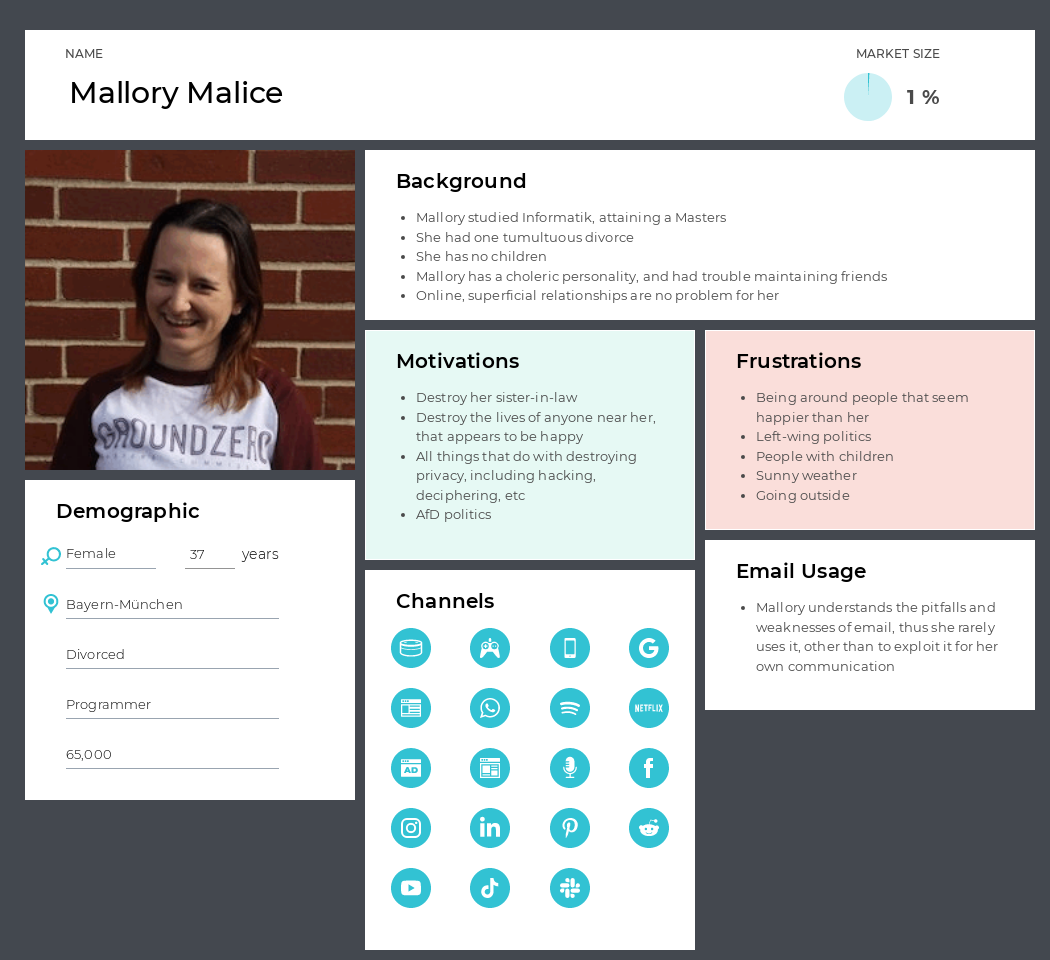
\includegraphics[scale=.38]{Mallory Malice.png}





%\section{Index} I don't know what purpose this is supposed to serve, and it's not clearly stated in the document, so I am leaving it out for now.

\backmatter

\clearpage % or \cleardoublepage
\addcontentsline{toc}{chapter}{References}

%new command added to change Bibliography title to References
\renewcommand{\bibname}{References}

\begin{thebibliography}{11}

\bibitem[Shirey, 2007]{Shirey}
  Shirey, R.,
  \emph{“RFC 4949 - Internet Security Glossary, Version 2.”},
  Document Search and Retrieval Page,
  Aug. 2007,
  https://datatracker.ietf.org/doc/html/rfc4949. 

\bibitem[Delfs and Knebl, 2002]{DelfsKnebl}
  Delfs, Hans, and Helmut Knebl,
  \emph{Introduction to Cryptography: Principles and Applications},
  p. 12, Springer Verlag, Berlin,
  2007.
  
\bibitem[Schneier, 2015]{Schneier}
  Schneier, Bruce,
  \emph{Applied Cryptography: Protocols, Algorithms, and Source Code in C},
  p. 155, Wiley, Indianapolis, IN,
  2015.

\bibitem[Nirula, 2022]{Nirula}
  Nirula, Urvashi,
  \emph{Block Cipher | Purpose, Applications \& Examples},
  Document Search and Retrieval Page,
  https://study.com/learn/lesson/block-cipher-purpose-applications.html
  
\bibitem[Aumasson, 2017]{Aumasson}
  Aumasson, Jean-Philippe,
  \emph{Serious cryptography: A practical introduction to modern encryption},
  p. 107, No Starch Press Inc, San Francisco, CA, 
  2017
  
\bibitem[Paar \& Pelzl, 2009]{PaarPelzl}
  Paar, Christof., \& Pelzl, J.,
 \emph{Understanding cryptography: A textbook for students and practitioners.},
  Springer Science \& Business Media,
  2009
  
\bibitem[Dooley, 2008]{Dooley}
  Dooley, J. F.,
  \emph{History of cryptography and cryptanalysis: Codes, ciphers, and their algorithms},
   Springer,
   2008
  
\bibitem[Katz \& Lindell, 2007]{Katz}
  Katz, J., \& Lindell, Y.,
  \emph{Introduction to modern cryptography: Principles and protocols},
  CRC Press,
  2007
  
\bibitem[Martin, 2017]{book10}
  Martin, K.,
  \emph{Everyday cryptography: Fundamental principles and applications},
  Oxford University Press,
  2017
  
\bibitem[Crawford, 2019]{Crawford}
  Crawford, Douglas.,
  \emph{“AES Encryption: Everything You Need to Know about AES.”},
   ProPrivacy.com, 
   4 Feb. 2019, 
   https://proprivacy.com/guides/aes-encryption. 

\bibitem[Stanford Security Lab, 2009]{SJCL}
  Stanford Security Lab,
  \emph {“Stanford Javascript Crypto Library (SJCL).”},
   SJCL: a Javascript Crypto Library, 
   Stanford University,
   https://crypto.stanford.edu/sjcl/.
   
\bibitem[Mozilla]{WebEx}
  Thunderbird Add-on Team.,
  “Introduction to Add-on Development.”,
  Thunderbird, Mozilla, 
  https://developer.thunderbird.net/add-ons/mailextensions. 
   

\end{thebibliography}


\end{document}